%----------------------------------------------------------------------------
%bb defines the bounding box for the pdf
%viewport defines the area of the pdf used
%in sidewaysfigure the last entry in bb moves the caption toward/away the pic
%in sidewaysfigure the second entry in bb moves the pic toward/away the caption
%----------------------------------------------------------------------------
\begin{figure}
\scalebox{0.8}[0.8]{
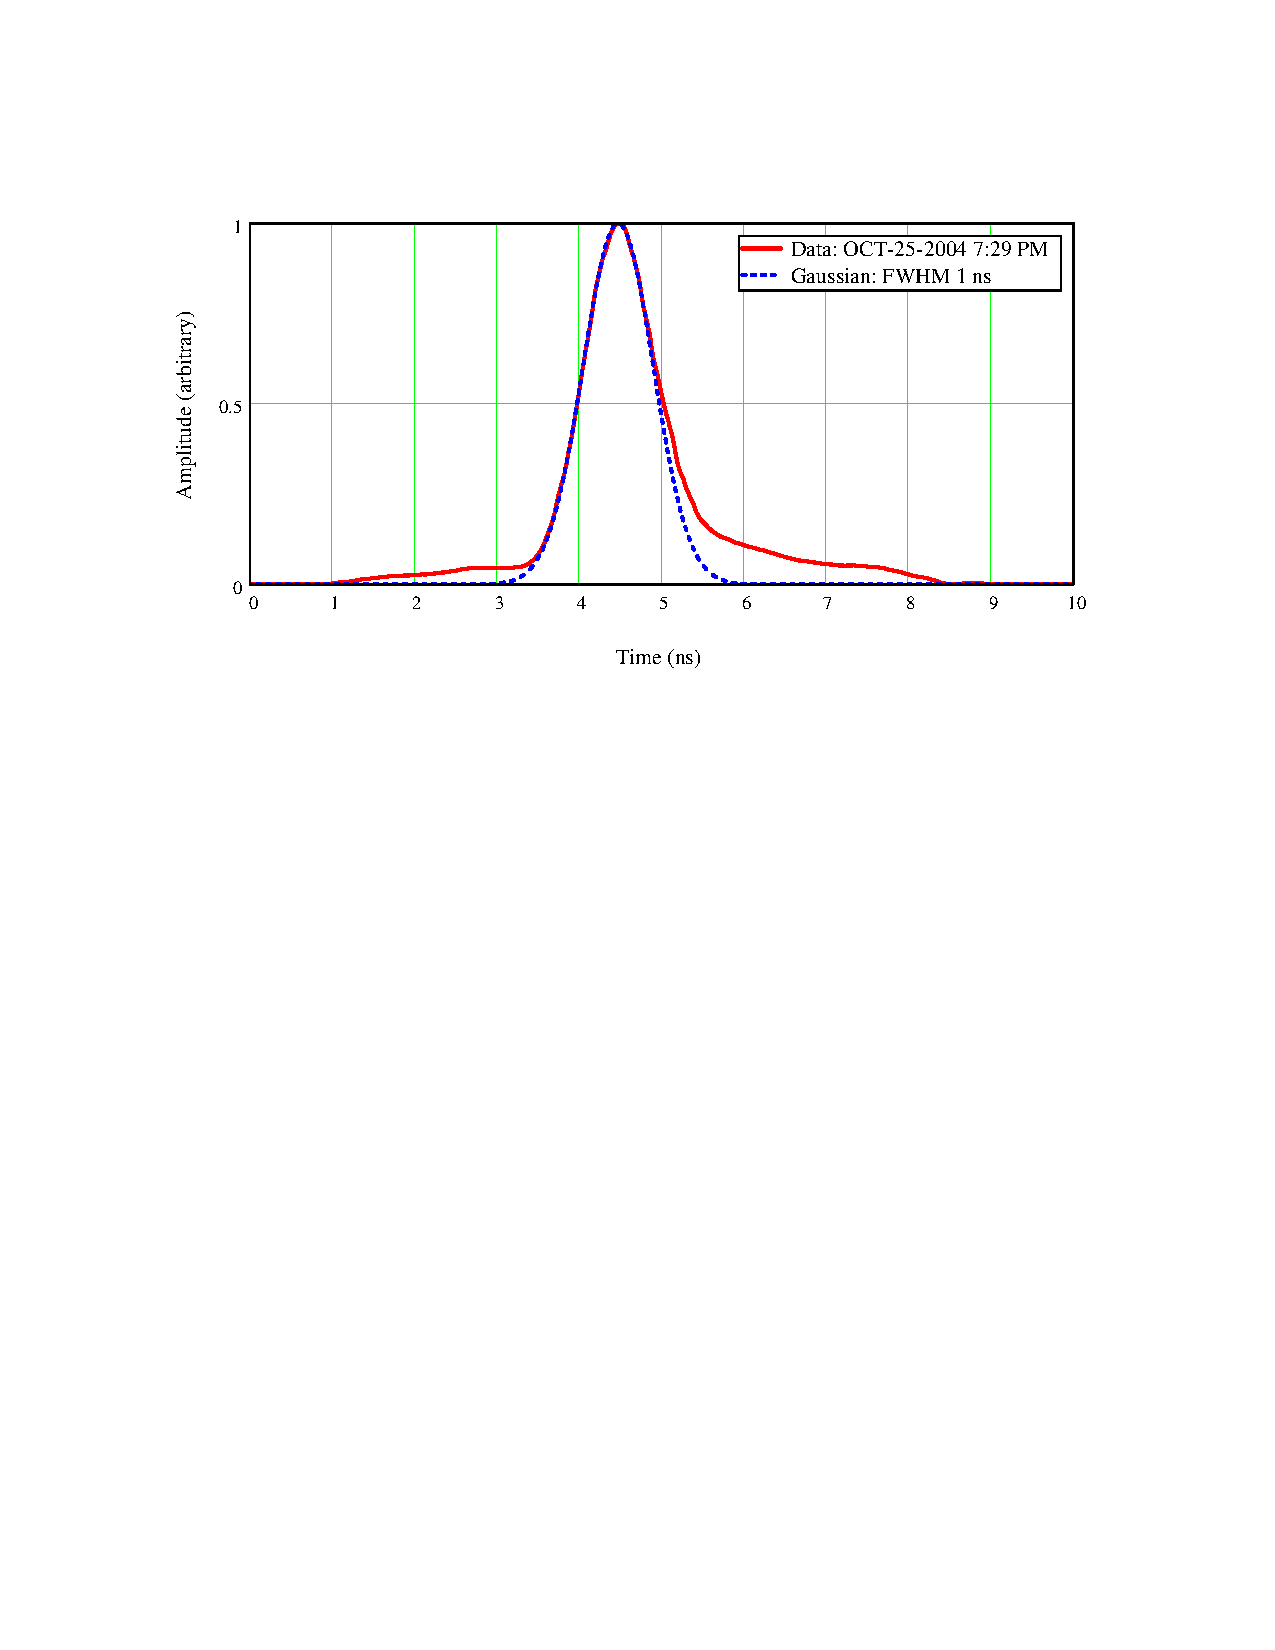
\includegraphics[bb=35 467 523 689]
{temporal_profiles/temporal_profiles.pdf}
}
\caption[Pockels cell minimum pulse length (temporal profiles)]{Pockels cell minimum pulse length (temporal profiles). Here the data corresponding to a 3'' delay cable is overlaid with a computer generated Gaussian pulse. There is significant leaking before and after the pulse; this perhaps due to the relatively low (manufacturer specified) extinction ratio of 1k:1 for the polarizers (compared to 10k:1 for the polarizers used in the HeNe test) and the mismatch between the design wavelength and the laser wavelength.}
\label{temporal profiles}
\end{figure}
%----------------------------------------------------------------------------
